\documentclass[a4paper,12pt]{article}

\usepackage[utf8x]{inputenc}
\usepackage[T2A]{fontenc}
\usepackage[english, russian]{babel}

% Опционно, требует  apt-get install scalable-cyrfonts.*
% и удаления одной строчки в cyrtimes.sty
% Сточку не удалять!
% \usepackage{cyrtimes}

% Картнки и tikz
\usepackage{graphicx}
\usepackage{tikz}
\usetikzlibrary{snakes,arrows,shapes}


% Некоторая русификация.
\usepackage{misccorr}
\usepackage{indentfirst}
\renewcommand{\labelitemi}{\normalfont\bfseries{--}}

% Увы, поля придётся уменьшить из-за листингов.
\topmargin -1cm
\oddsidemargin -0.5cm
\evensidemargin -0.5cm
\textwidth 17cm
\textheight 24cm

\sloppy

% Оглавление в PDF
\usepackage[
bookmarks=true,
colorlinks=true, linkcolor=black, anchorcolor=black, citecolor=black, menucolor=black,filecolor=black, urlcolor=black,
unicode=true
]{hyperref}

% Для исходного кода в тексте
\newcommand{\Code}[1]{\texttt{#1}}


\title{Отчёт по лабораторной работе \\ <<IP-маршрутизация>>}
\author{Здесь Ф.~И.~О}

\begin{document}

\maketitle

\tableofcontents

% Текст отчёта должен быть читаемым!!! Написанное здесь является рыбой.

\section{Топология сети}

Топология сети и использыемые IP-адреса показаны на рис.~\ref{fig:network}.

\begin{figure}
\centering
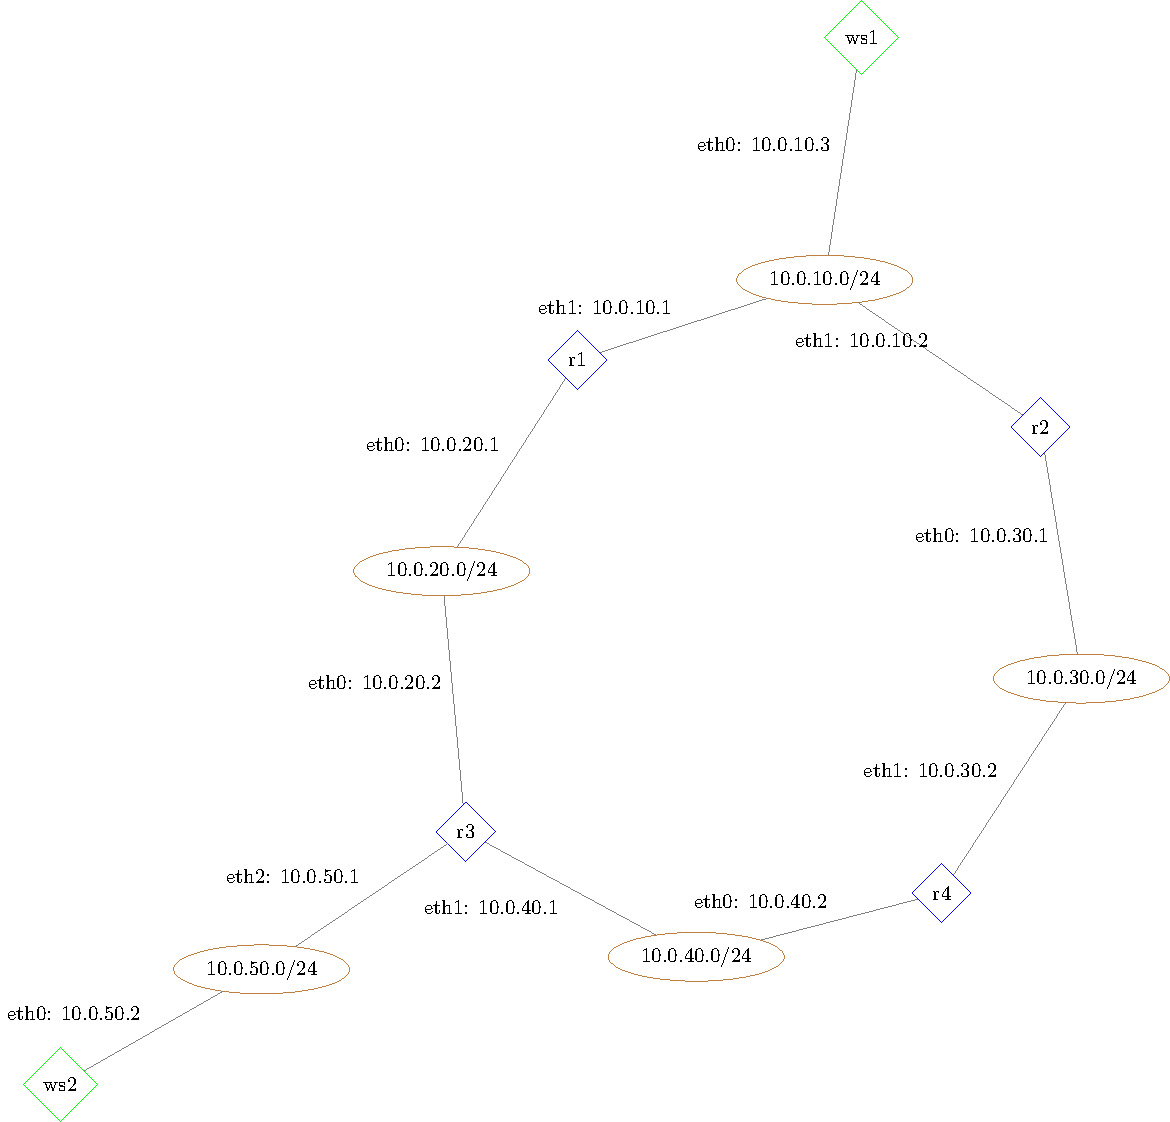
\includegraphics[width=\textwidth]{includes/network_gv.pdf}
\caption{Топология сети}
\label{fig:network}
\end{figure}


\section{Назначение IP-адресов}

Ниже приведён файл настройки протокола IP маршрутизатора r1

\begin{Verbatim}
    auto lo
    iface lo inet loopback
    
    auto eth0
    iface eth0 inet static
    address 10.0.20.1
    netmask 255.255.255.0
    up ip r add 10.0.40.0/24 via 10.0.20.2 dev eth0
    up ip r add 10.0.50.0/24 via 10.0.20.2 dev eth0
    down ip r del 10.0.40.0/24
    down ip r del 10.0.50.0/24
    
    auto eth1
    iface eth1 inet static
    address 10.0.10.1
    netmask 255.255.255.0
    up ip r add 10.0.30.0/24 via 10.0.10.2 dev eth1
    down ip r del 10.0.30.0/24
\end{Verbatim}

Ниже приведён файл настройки протокола IP маршрутизатора r1

\begin{Verbatim}
auto lo
iface lo inet loopback

auto eth0
iface eth0 inet static
address 10.0.30.1
netmask 255.255.255.0
up ip r add 10.0.40.0/24 via 10.0.30.2 dev eth0
down ip r del 10.0.40.0/24

auto eth1
iface eth1 inet static
address 10.0.10.2
netmask 255.255.255.0
up ip r add 10.0.20.0/24 via 10.0.10.1 dev eth1
up ip r add 10.0.50.0/24 via 10.0.10.1 dev eth1
down ip r del 10.0.20.0/24
down ip r del 10.0.50.0/24
\end{Verbatim}

Ниже приведён файл настройки протокола IP маршрутизатора r1

\begin{Verbatim}
auto lo
iface lo inet loopback

auto eth0
iface eth0 inet static
address 10.0.20.2
netmask 255.255.255.0
up ip r add 10.0.10.0/24 via 10.0.20.1 dev eth0
down ip r del 10.0.10.0/24

auto eth1
iface eth1 inet static
address 10.0.40.1
netmask 255.255.255.0
up ip r add 10.0.30.0/24 via 10.0.40.2 dev eth1
down ip r del 10.0.30.0/24

auto eth2
iface eth2 inet static
address 10.0.50.1
netmask 255.255.255.0
\end{Verbatim}

Ниже приведён файл настройки протокола IP маршрутизатора r1

\begin{Verbatim}
auto lo
iface lo inet loopback

auto eth0
iface eth0 inet static
address 10.0.40.2
netmask 255.255.255.0
up ip r add 10.0.20.0/24 via 10.0.40.1 dev eth0
up ip r add 10.0.50.0/24 via 10.0.40.1 dev eth0
down ip r del 10.0.20.0/24
down ip r del 10.0.50.0/24

auto eth1
iface eth1 inet static
address 10.0.30.2
netmask 255.255.255.0
up ip r add 10.0.10.0/24 via 10.0.30.1 dev eth1
down ip r del 10.0.10.0/24
\end{Verbatim}

Ниже приведён файл настройки протокола IP рабочей станции ws1.

\begin{Verbatim}
auto lo
iface lo inet loopback

auto eth0
iface eth0 inet static
address 10.0.10.3
netmask 255.255.255.0
gateway 10.0.10.2
\end{Verbatim}

Ниже приведён файл настройки протокола IP рабочей станции ws2.

\begin{Verbatim}
auto lo
iface lo inet loopback

auto eth0
iface eth0 inet static
address 10.0.50.2
netmask 255.255.255.0
gateway 10.0.50.1
\end{Verbatim}


\section{Таблица маршрутизации}

Вывести (командой ip r) таблицу маршрутизации для \textbf{r1}.

\begin{Verbatim}
r1:~# ip r
10.0.20.0/24 dev eth0  proto kernel  scope link  src 10.0.20.1 
10.0.50.0/24 via 10.0.20.2 dev eth0 
10.0.30.0/24 via 10.0.10.2 dev eth1 
10.0.40.0/24 via 10.0.20.2 dev eth0 
10.0.10.0/24 dev eth1  proto kernel  scope link  src 10.0.10.1
\end{Verbatim}

Вывести (командой ip r) таблицу маршрутизации для \textbf{r2}.

\begin{Verbatim}
r2:~# ip r
10.0.20.0/24 via 10.0.10.1 dev eth1 
10.0.50.0/24 via 10.0.10.1 dev eth1 
10.0.30.0/24 dev eth0  proto kernel  scope link  src 10.0.30.1 
10.0.40.0/24 via 10.0.30.2 dev eth0 
10.0.10.0/24 dev eth1  proto kernel  scope link  src 10.0.10.2 
\end{Verbatim}

Вывести (командой ip r) таблицу маршрутизации для \textbf{r3}.

\begin{Verbatim}
r3:~# ip r
10.0.20.0/24 dev eth0  proto kernel  scope link  src 10.0.20.2 
10.0.50.0/24 dev eth2  proto kernel  scope link  src 10.0.50.1 
10.0.30.0/24 via 10.0.40.2 dev eth1 
10.0.40.0/24 dev eth1  proto kernel  scope link  src 10.0.40.1 
10.0.10.0/24 via 10.0.20.1 dev eth0 
\end{Verbatim}

Вывести (командой ip r) таблицу маршрутизации для \textbf{r4}.

\begin{Verbatim}
r4:~# ip r
10.0.20.0/24 via 10.0.40.1 dev eth0 
10.0.50.0/24 via 10.0.40.1 dev eth0 
10.0.30.0/24 dev eth1  proto kernel  scope link  src 10.0.30.2 
10.0.40.0/24 dev eth0  proto kernel  scope link  src 10.0.40.2 
10.0.10.0/24 via 10.0.30.1 dev eth1 
\end{Verbatim}

Вывести (командой ip r) таблицу маршрутизации для \textbf{ws1}.

\begin{Verbatim}
ws1:~# ip r
10.0.10.0/24 dev eth0  proto kernel  scope link  src 10.0.10.3 
default via 10.0.10.1 dev eth0 
\end{Verbatim}

Вывести (командой ip r) таблицу маршрутизации для \textbf{ws2}.

\begin{Verbatim}
ws2:~# ip r
10.0.50.0/24 dev eth0  proto kernel  scope link  src 10.0.50.2 
default via 10.0.50.1 dev eth0
\end{Verbatim}

% ... Повторять для всех маршрутизаторов и рабочих станций, где есть что-то кроме gateway.

\section{Проверка настройки сети}

Вывод \textbf{traceroute} от узла такого-то до такого-то при нормальной работе сети.

\begin{Verbatim}
ws1:~# traceroute -n 10.0.50.2
traceroute to 10.0.50.2 (10.0.50.2), 64 hops max, 40 byte packets
 1  10.0.10.1  8 ms  0 ms  0 ms
 2  10.0.20.2  11 ms  0 ms  1 ms
 3  10.0.50.2  12 ms  3 ms  2 ms
\end{Verbatim}

\section{Маршрутизация}

% На пути здесь достаточно быть одному аршрутизатору!

Вначале стоит написать, какие MAC-адреса интерфейсов в опыте были у каких машин.
Затем вывести маршрутную таблицу маршрутизатора (вывод команды ip r!)

MAC адреса интерфейсов маршрутизатора r1
\begin{Verbatim}
r1:~# ip link
1: lo: <LOOPBACK,UP,LOWER_UP> mtu 16436 qdisc noqueue 
    link/loopback 00:00:00:00:00:00 brd 00:00:00:00:00:00
2: teql0: <NOARP> mtu 1500 qdisc noop qlen 100
    link/void 
3: eth0: <BROADCAST,MULTICAST,UP,LOWER_UP> mtu 1500 qdisc pfifo_fast qlen 1000
    link/ether 0e:ab:f8:0c:10:4b brd ff:ff:ff:ff:ff:ff
4: eth1: <BROADCAST,MULTICAST,UP,LOWER_UP> mtu 1500 qdisc pfifo_fast qlen 1000
    link/ether fa:de:dc:30:96:57 brd ff:ff:ff:ff:ff:ff
\end{Verbatim}

MAC адреса интерфейсов маршрутизатора r3
\begin{Verbatim}
r3:~# ip link
1: lo: <LOOPBACK,UP,LOWER_UP> mtu 16436 qdisc noqueue 
    link/loopback 00:00:00:00:00:00 brd 00:00:00:00:00:00
2: teql0: <NOARP> mtu 1500 qdisc noop qlen 100
    link/void 
3: eth0: <BROADCAST,MULTICAST,UP,LOWER_UP> mtu 1500 qdisc pfifo_fast qlen 1000
    link/ether ee:97:f2:ab:47:0c brd ff:ff:ff:ff:ff:ff
4: eth1: <BROADCAST,MULTICAST,UP,LOWER_UP> mtu 1500 qdisc pfifo_fast qlen 1000
    link/ether d2:90:43:d2:95:19 brd ff:ff:ff:ff:ff:ff
5: eth2: <BROADCAST,MULTICAST,UP,LOWER_UP> mtu 1500 qdisc pfifo_fast qlen 1000
    link/ether c2:57:e2:f3:3f:00 brd ff:ff:ff:ff:ff:ff
\end{Verbatim}

MAC адреса интерфейсов рабочей станции ws1
\begin{Verbatim}
ws1:~# ip link
1: lo: <LOOPBACK,UP,LOWER_UP> mtu 16436 qdisc noqueue 
    link/loopback 00:00:00:00:00:00 brd 00:00:00:00:00:00
2: teql0: <NOARP> mtu 1500 qdisc noop qlen 100
    link/void 
3: eth0: <BROADCAST,MULTICAST,UP,LOWER_UP> mtu 1500 qdisc pfifo_fast qlen 1000
    link/ether a6:f9:52:b6:1e:69 brd ff:ff:ff:ff:ff:ff
\end{Verbatim}

MAC адреса интерфейсов рабочей станции ws2
\begin{Verbatim}
ws2:~# ip link
1: lo: <LOOPBACK,UP,LOWER_UP> mtu 16436 qdisc noqueue 
    link/loopback 00:00:00:00:00:00 brd 00:00:00:00:00:00
2: teql0: <NOARP> mtu 1500 qdisc noop qlen 100
    link/void 
3: eth0: <BROADCAST,MULTICAST,UP,LOWER_UP> mtu 1500 qdisc pfifo_fast qlen 1000
    link/ether da:53:12:09:ea:4e brd ff:ff:ff:ff:ff:ff
\end{Verbatim}

Показаны опыты после стирания кеша ARP.
% Не забудьте это сделать!
Далее показана отправка пакета на маршрутизатор (косвенная маршрутизация). 
fff
tcpdump на маршрутизаторе r1
\begin{Verbatim}
r1:~# tcpdump -tne -i eth1
tcpdump: verbose output suppressed, use -v or -vv for full protocol decode
listening on eth1, link-type EN10MB (Ethernet), capture size 96 bytes
a6:f9:52:b6:1e:69 > ff:ff:ff:ff:ff:ff, ethertype ARP (0x0806), length 42: arp who-has 10.0.10.1 tell 10.0.10.3
fa:de:dc:30:96:57 > a6:f9:52:b6:1e:69, ethertype ARP (0x0806), length 42: arp reply 10.0.10.1 is-at fa:de:dc:30:96:57
a6:f9:52:b6:1e:69 > fa:de:dc:30:96:57, ethertype IPv4 (0x0800), length 98: 10.0.10.3 > 10.0.50.2: ICMP echo request, id 18178, seq 1, length 64
fa:de:dc:30:96:57 > a6:f9:52:b6:1e:69, ethertype IPv4 (0x0800), length 98: 10.0.50.2 > 10.0.10.3: ICMP echo reply, id 18178, seq 1, length 64
fa:de:dc:30:96:57 > a6:f9:52:b6:1e:69, ethertype ARP (0x0806), length 42: arp who-has 10.0.10.3 tell 10.0.10.1
a6:f9:52:b6:1e:69 > fa:de:dc:30:96:57, ethertype ARP (0x0806), length 42: arp reply 10.0.10.3 is-at a6:f9:52:b6:1e:69
\end{Verbatim}

Затем маршрутизатор отправил его далее.

tcpdump на маршрутизаторе r3
\begin{Verbatim}
    привет
r3:~# tcpdump -tne
tcpdump: verbose output suppressed, use -v or -vv for full protocol decode
listening on eth0, link-type EN10MB (Ethernet), capture size 96 bytes
0e:ab:f8:0c:10:4b > ff:ff:ff:ff:ff:ff, ethertype ARP (0x0806), length 42: arp who-has 10.0.20.2 tell 10.0.20.1
ee:97:f2:ab:47:0c > 0e:ab:f8:0c:10:4b, ethertype ARP (0x0806), length 42: arp reply 10.0.20.2 is-at ee:97:f2:ab:47:0c
0e:ab:f8:0c:10:4b > ee:97:f2:ab:47:0c, ethertype IPv4 (0x0800), length 98: 10.0.10.3 > 10.0.50.2: ICMP echo request, id 18178, seq 1, length 64
ee:97:f2:ab:47:0c > 0e:ab:f8:0c:10:4b, ethertype IPv4 (0x0800), length 98: 10.0.50.2 > 10.0.10.3: ICMP echo reply, id 18178, seq 1, length 64
ee:97:f2:ab:47:0c > 0e:ab:f8:0c:10:4b, ethertype ARP (0x0806), length 42: arp who-has 10.0.20.1 tell 10.0.20.2
0e:ab:f8:0c:10:4b > ee:97:f2:ab:47:0c, ethertype ARP (0x0806), length 42: arp reply 10.0.20.1 is-at 0e:ab:f8:0c:10:4b
\end{Verbatim}

tcpdump на рабочей станции ws2
\begin{Verbatim}
ws2:~# tcpdump -tne
tcpdump: verbose output suppressed, use -v or -vv for full protocol decode
listening on eth0, link-type EN10MB (Ethernet), capture size 96 bytes
c2:57:e2:f3:3f:00 > ff:ff:ff:ff:ff:ff, ethertype ARP (0x0806), length 42: arp who-has 10.0.50.2 tell 10.0.50.1
da:53:12:09:ea:4e > c2:57:e2:f3:3f:00, ethertype ARP (0x0806), length 42: arp reply 10.0.50.2 is-at da:53:12:09:ea:4e
c2:57:e2:f3:3f:00 > da:53:12:09:ea:4e, ethertype IPv4 (0x0800), length 1042: 10.0.10.3 > 10.0.50.2: ICMP echo request, id 17922, seq 1, length 1008
da:53:12:09:ea:4e > c2:57:e2:f3:3f:00, ethertype IPv4 (0x0800), length 1042: 10.0.50.2 > 10.0.10.3: ICMP echo reply, id 17922, seq 1, length 1008
da:53:12:09:ea:4e > c2:57:e2:f3:3f:00, ethertype ARP (0x0806), length 42: arp who-has 10.0.50.1 tell 10.0.50.2
c2:57:e2:f3:3f:00 > da:53:12:09:ea:4e, ethertype ARP (0x0806), length 42: arp reply 10.0.50.1 is-at c2:57:e2:f3:3f:00

\end{Verbatim}

\section{Продолжительность жизни пакета}

Для того чтобы отследить продолжительность жизни отправленного пакета на маршрутизаторе r3 был выключен интерфей eth2 в сети 10.0.50.0/24 и добавлен неверный маршрут

\begin{Verbatim}
r3:~# ip link set eth2 down
r3:~# ip route add 10.0.50.0/24 via 10.0.20.1 dev eth0
\end{Verbatim}

Таблица маршрутизации в r3

\begin{Verbatim}
r3:~# ip r
10.0.20.0/24 dev eth0  proto kernel  scope link  src 10.0.20.2 
10.0.50.0/24 via 10.0.20.1 dev eth0 
10.0.30.0/24 via 10.0.40.2 dev eth1 
10.0.40.0/24 dev eth1  proto kernel  scope link  src 10.0.40.1 
10.0.10.0/24 via 10.0.20.1 dev eth0 
\end{Verbatim}

Из-за истечения ttl появляется ошибка

\begin{Verbatim}
ws1:~# ping 10.0.50.2
PING 10.0.50.2 (10.0.50.2) 56(84) bytes of data.
From 10.0.20.2 icmp_seq=1 Time to live exceeded
\end{Verbatim}

\section{Изучение IP-фрагментации}

Установим в интерфейсах, подключенных к сети 10.0.20.0/24 MTU=576

Маршрутизатор r1
\begin{Verbatim}
r1:~# ip link set dev eth0 mtu 576
r1:~# ip l
1: lo: <LOOPBACK,UP,LOWER_UP> mtu 16436 qdisc noqueue 
    link/loopback 00:00:00:00:00:00 brd 00:00:00:00:00:00
2: teql0: <NOARP> mtu 1500 qdisc noop qlen 100
    link/void 
3: eth0: <BROADCAST,MULTICAST,UP,LOWER_UP> mtu 576 qdisc pfifo_fast qlen 1000
    link/ether 0e:ab:f8:0c:10:4b brd ff:ff:ff:ff:ff:ff
4: eth1: <BROADCAST,MULTICAST,UP,LOWER_UP> mtu 1500 qdisc pfifo_fast qlen 1000
    link/ether fa:de:dc:30:96:57 brd ff:ff:ff:ff:ff:ff
r1:~# 
\end{Verbatim}

Маршрутизатор r3
\begin{Verbatim}
r3:~# ip link set dev eth0 mtu 576
r3:~# ip l
1: lo: <LOOPBACK,UP,LOWER_UP> mtu 16436 qdisc noqueue 
    link/loopback 00:00:00:00:00:00 brd 00:00:00:00:00:00
2: teql0: <NOARP> mtu 1500 qdisc noop qlen 100
    link/void 
3: eth0: <BROADCAST,MULTICAST,UP,LOWER_UP> mtu 576 qdisc pfifo_fast qlen 1000
    link/ether ee:97:f2:ab:47:0c brd ff:ff:ff:ff:ff:ff
4: eth1: <BROADCAST,MULTICAST,UP,LOWER_UP> mtu 1500 qdisc pfifo_fast qlen 1000
    link/ether d2:90:43:d2:95:19 brd ff:ff:ff:ff:ff:ff
5: eth2: <BROADCAST,MULTICAST,UP,LOWER_UP> mtu 1500 qdisc pfifo_fast qlen 1000
    link/ether c2:57:e2:f3:3f:00 brd ff:ff:ff:ff:ff:ff
\end{Verbatim}

Выключаем защиту от фрагментации PMTU на машине ws1

\begin{Verbatim}
echo 1 > /proc/sys/net/ipv4/ip_no_pmtu_disc
\end{Verbatim}
% Напоминаем, что PMTU следует отключить!

Посылаем эхо запрос с пакетом величиной 1000 

\begin{Verbatim}
ping -c 1 -s 1000 10.0.50.2
\end{Verbatim}

На маршрутизатор r1 приходит целый пакет

\begin{Verbatim}
r1:~# tcpdump -tnv -i eth1 icmp
tcpdump: listening on eth1, link-type EN10MB (Ethernet), capture size 96 bytes
IP (tos 0x0, ttl 64, id 25781, offset 0, flags [none], proto ICMP (1), length 1028) 10.0.10.3 > 10.0.50.2: ICMP echo request, id 18946, seq 1, length 1008
IP (tos 0x0, ttl 62, id 28225, offset 0, flags [none], proto ICMP (1), length 1028) 10.0.50.2 > 10.0.10.3: ICMP echo reply, id 18946, seq 1, length 1008
\end{Verbatim}

Для дальнешей передаче пакета он фрагментируется на 2 пакета меньшего размера, это видно на маршрутизаторе r3 - туда пришло 2 пакета
% Вывод в ширину можно и сократить, удалив несущественные моменты!

\begin{Verbatim}
r3:~# tcpdump -tnv -i eth0 icmp
tcpdump: listening on eth0, link-type EN10MB (Ethernet), capture size 96 bytes
IP (tos 0x0, ttl 63, id 25781, offset 0, flags [+], proto ICMP (1), length 572) 10.0.10.3 > 10.0.50.2: ICMP echo request, id 18946, seq 1, length 552
IP (tos 0x0, ttl 63, id 25781, offset 552, flags [none], proto ICMP (1), length 476) 10.0.10.3 > 10.0.50.2: icmp
IP (tos 0x0, ttl 63, id 28225, offset 0, flags [+], proto ICMP (1), length 572) 10.0.50.2 > 10.0.10.3: ICMP echo reply, id 18946, seq 1, length 552
IP (tos 0x0, ttl 63, id 28225, offset 552, flags [none], proto ICMP (1), length 476) 10.0.50.2 > 10.0.10.3: icmp
\end{Verbatim}
При передаче пакета на машину ws2 в сеть 10.0.50.0/24 пакет был дефрагментирован на маршрутизаторе r3, так как в интерфейсе, подключенному к этой сети, величина MTU=1500

\begin{Verbatim}
ws2:~# tcpdump -tnv -i eth0 icmp
tcpdump: listening on eth0, link-type EN10MB (Ethernet), capture size 96 bytes
IP (tos 0x0, ttl 62, id 25781, offset 0, flags [none], proto ICMP (1), length 1028) 10.0.10.3 > 10.0.50.2: ICMP echo request, id 18946, seq 1, length 1008
IP (tos 0x0, ttl 64, id 28225, offset 0, flags [none], proto ICMP (1), length 1028) 10.0.50.2 > 10.0.10.3: ICMP echo reply, id 18946, seq 1, length 1008
\end{Verbatim}


\section{Отсутствие сети}

Аналогично опишите опыт, когда маршрутизатор отсылает сообщение об отстутствии с сети.
С командами и выводом, мак адреса не нужны.

\begin{Verbatim}
ws1:~# ping 10.0.60.2 -c 1
PING 10.0.60.2 (10.0.60.2) 56(84) bytes of data.
From 10.0.10.1 icmp_seq=1 Destination Net Unreachable

--- 10.0.60.2 ping statistics ---
1 packets transmitted, 0 received, +1 errors, 100% packet loss, time 0ms
\end{Verbatim}


\section{Отсутствие IP-адреса в сети}

Аналогично опишите опыт, когда маршрутизатор отсылает сообщение об отстутствии требуемого IP-адреса в сети.
С командами и выводом, мак адреса не нужны.

\begin{Verbatim}
ws1:~# ping 10.0.50.3 -c 1
PING 10.0.50.3 (10.0.50.3) 56(84) bytes of data.
From 10.0.20.2 icmp_seq=1 Destination Host Unreachable

--- 10.0.50.3 ping statistics ---
1 packets transmitted, 0 received, +1 errors, 100% packet loss, time 0ms
\end{Verbatim}

\end{document}
